
\chapter{失智症之認知功能評估}
\label{chapter:intro}


\begin{figure}[H]
	\centering
	\centerline{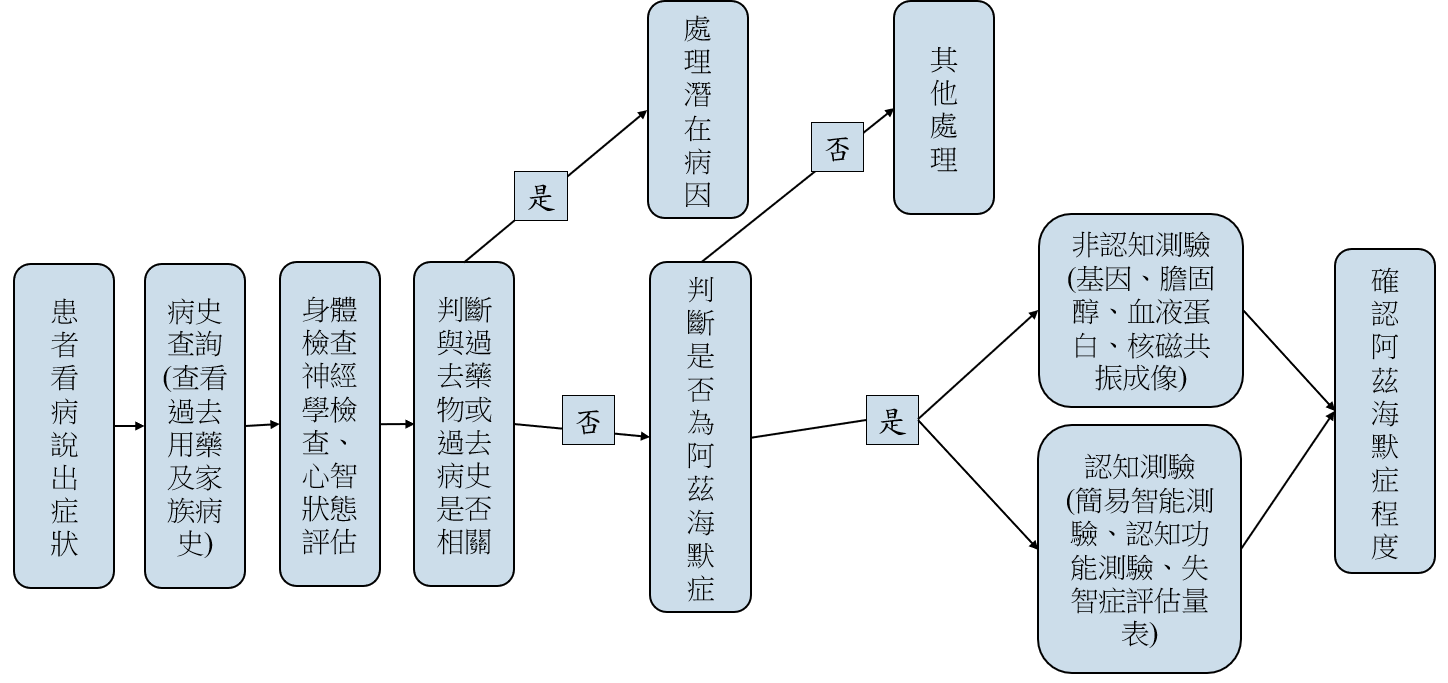
\includegraphics[height=8cm]{pic/ADprocess.PNG}}
	\label{fig:ADProcess}
\end{figure}

\section{臨床失智評估表(Clinical Dementia Rating,CDR)}

具有輕微認知症狀(例如記憶力下降)的患者是否患有前期或臨床前阿茲海默氏病(Alzheimer disease,AD)並在不久的將來發展為 AD 癡呆仍然是臨床醫生面臨的挑戰。這項任務對於正確和早期的 AD 診斷、開始對AD症治療、規劃未來以及希望很快開始改善疾病的治療都至關重要。

美國華盛頓大學的Hughes等人提出,用來評估阿茲海默 症患者日常生活及認知功能作整體性評估的量表。
用來對阿茲海默症患者,日常生活與認知功能作整體性評估的量表,是評估失智症嚴重程度的主要工具。隨著病程變化,某些特定日常生活功能會先出現障礙,當病程逐漸變嚴重時,其他不同日常生活障礙也陸續出現。藉由區分患者日常生活與認知功能障礙的程度,作為判定阿茲海默症嚴重程度的依據。


CDR包含有6個功能項目:記憶、定向力、判斷與解決問題、社區事務、家居與嗜好、個人照料
對上述的6個功能項目,分為0\~3 的5個不同功能程度

\begin{itemize}
    \item
    0 代表健康 (Health)
    \item
    0.5 代表疑似或輕微障礙 (Questionable)
    \item
    1 代表輕度障礙 (Mild)
    \item
    2 代表中度障礙 (Moderate)
    \item
    3 代表重度障礙 (Severe)
\end{itemize}

\clearpage
CDR是一個半結構性晤談的評估,主要包
括兩個部份:
\begin{enumerate}
	\item
受試者部份:針對各種認知功能範圍,包括有注意力、長期記憶、近期記憶、時空定向力、語言、抽象與判斷等作評估。
\item
家人部份:詢問患者家人或主要照顧者,就受試者在日常生活上,是否有出現與記憶力有關的問題或困擾。
\end{enumerate}

\begin{figure}[H]
	\centering
	\centerline{\includegraphics[height=20cm]{pic/CDR.PNG}}
	\caption{CDR 臨床失智評分量表}
	\begin{minipage}{.7\linewidth}

		\footnotesize
		\emph{來源:}衛生福利部,失智症診療手冊

	\end{minipage}
	\label{fig:CDR}
\end{figure}

\section{簡易智能評估(Mini-Mental State Examination,MMSE)}
為臨床上最廣泛應用評估老年人認知狀態之工具,共分為定向感、記錄能力、注意力和計算力、回憶能力、抽象概念和語言能力來評估,滿分是三十分,答對一項給一分,若低於二十三分表度知能損傷,低於十六分表重度認知功能損傷。


是Folstein等人1975年所提出,2001年3月MMSE版權已轉為PAR, Inc.所有,任何臨床上使用、論文發表及研究使用需至PAR,Inc.網站申請版權使用。

MMSE (總分 30分) 包括五大施測項目 (下列括號中的數字為最高得分):
\begin{enumerate}
	\item
    定向感(10分):分為 時間定向力 (5分) 與 地點定向力 (5分) 兩部分。
	\item
	訊息登錄 (3分): 目的是要受試者學習三樣東西,稍後要作為短期回憶的測試使用。
	\item
	注意力與算術能力(5分):請受試者由 100 減 7 等於? 再減 7 等於?...連續進行五次。
	\item
    立即記憶與短期記憶(3分):詢問受試者是否記得先前重述的三樣東西 (順序無所謂)。
	\item
	語言理解、空間概念、與操作能力 (9分): 
	
	包含下列的問題:
	\begin{itemize}
		\item
		兩個一般常用物品的命名 (2分)。
		\item
		請受試者重述一個句子 (1分)。
		\item
		請受試者讀 “請閉上眼睛” 並做出動作(1分)。
		\item
		請受試者造一個句子並把它寫出來 (1分)。
		\item
		請受試者抄繪兩個五邊型其交叉為四邊型的圖形 (1分)。 
		\item
		請受試者在聽完 “用你的左手來拿這張紙,將它對折一半,然後交還給我” 的題目
後依序做出動作 (3分)。
	\end{itemize}

\end{enumerate}




\section{神經心理衡鑑(CASI)}
認知功能障礙篩檢量表 (CASI):經由固定的換算方式可以把它化成9個認知功能的細項,分別是長期記憶、注意力、時空定向力、語言能力、思緒流暢度、近期記憶、集中與心算力、抽象與判斷、空間概念
與構圖。

測驗總分100分,也可用於推估MMSE分數,MMSE施測的重要事項也可應用於CASI施測,CAIS會受教育程度與年齡影響。





%\section{附錄:MMSE和CDR}

%\includepdf[pages={1,2,3,4,5,6,7,8,9,10,11}]{MMSE.pdf}

%\includepdf[pages={1,2,3,4,5,6,7,8}]{CDR.pdf}
